% Options for packages loaded elsewhere
\PassOptionsToPackage{unicode}{hyperref}
\PassOptionsToPackage{hyphens}{url}
\documentclass[
]{article}
\usepackage{xcolor}
\usepackage{amsmath,amssymb}
\setcounter{secnumdepth}{-\maxdimen} % remove section numbering
\usepackage{iftex}
\ifPDFTeX
  \usepackage[T1]{fontenc}
  \usepackage[utf8]{inputenc}
  \usepackage{textcomp} % provide euro and other symbols
\else % if luatex or xetex
  \usepackage{unicode-math} % this also loads fontspec
  \defaultfontfeatures{Scale=MatchLowercase}
  \defaultfontfeatures[\rmfamily]{Ligatures=TeX,Scale=1}
\fi
\usepackage{lmodern}
\ifPDFTeX\else
  % xetex/luatex font selection
\fi
% Use upquote if available, for straight quotes in verbatim environments
\IfFileExists{upquote.sty}{\usepackage{upquote}}{}
\IfFileExists{microtype.sty}{% use microtype if available
  \usepackage[]{microtype}
  \UseMicrotypeSet[protrusion]{basicmath} % disable protrusion for tt fonts
}{}
\makeatletter
\@ifundefined{KOMAClassName}{% if non-KOMA class
  \IfFileExists{parskip.sty}{%
    \usepackage{parskip}
  }{% else
    \setlength{\parindent}{0pt}
    \setlength{\parskip}{6pt plus 2pt minus 1pt}}
}{% if KOMA class
  \KOMAoptions{parskip=half}}
\makeatother
\usepackage{longtable,booktabs,array}
\usepackage{caption}
\captionsetup[table]{skip=6pt}
\newcounter{none} % for unnumbered tables
\usepackage{calc} % for calculating minipage widths
% Correct order of tables after \paragraph or \subparagraph
\usepackage{etoolbox}
\makeatletter
\patchcmd\longtable{\par}{\if@noskipsec\mbox{}\fi\par}{}{}
\makeatother
\setlength{\emergencystretch}{3em} % prevent overfull lines
\providecommand{\tightlist}{%
  \setlength{\itemsep}{0pt}\setlength{\parskip}{0pt}}
\usepackage{bookmark}
\IfFileExists{xurl.sty}{\usepackage{xurl}}{} % add URL line breaks if available
\urlstyle{same}
% fallback for those not using the hyperref driver hyperxmp:
\makeatletter
\@ifundefined{xmpquote}{\newcommand{\xmpquote}[1]{#1}}{}
\makeatother
\hypersetup{
  hidelinks,
  pdfcreator={LaTeX via pandoc}}

\author{}
\date{}

\usepackage{graphicx}
\usepackage[a4paper, margin=0.85in]{geometry}
\usepackage{titlesec}
\usepackage{enumitem}
\usepackage{microtype}
\usepackage{fancyhdr}
\usepackage{ragged2e}
\usepackage{float}
\usepackage{setspace}
\usepackage{pdflscape}
\definecolor{gridsenseblue}{HTML}{174A6E}
\definecolor{gridsenselight}{HTML}{EAF1F5}
\titleformat{\section}{\Large\bfseries\color{gridsenseblue}}{}{0pt}{}
\titleformat{\subsection}{\large\bfseries\color{gridsenseblue}}{}{0pt}{}
\titleformat{\subsubsection}{\normalsize\bfseries\color{gridsenseblue}}{}{0pt}{}
\titlespacing*{\section}{0pt}{2.0ex plus .5ex minus .2ex}{1.0ex}
\titlespacing*{\subsection}{0pt}{1.7ex plus .4ex minus .2ex}{.7ex}
\titlespacing*{\subsubsection}{0pt}{1.4ex plus .3ex minus .2ex}{.5ex}
\setlist{nosep,leftmargin=2em}
\setlength{\parskip}{5pt plus 1pt minus 1pt}
\setlength{\parindent}{0pt}
\setlength{\emergencystretch}{4em}
\setlength{\LTpre}{8pt}
\setlength{\LTpost}{8pt}
\captionsetup{font=small,labelfont=bf}
\pagestyle{fancy}
\fancyhf{}
\fancyhead[L]{\small\textcolor{gridsenseblue}{GridSense}}
\fancyhead[R]{\small\thepage}
\renewcommand{\headrulewidth}{0.4pt}
\setlength{\headheight}{14pt}

\begin{document}

\begin{center}
\parbox{\textwidth}{\centering\LARGE\bfseries\color{gridsenseblue}
GridSense: Smart EV Charging and Load Management\par}
\vspace{0.6em}
\end{center}
\label{gridsense-smart-ev-charging-and-load-management}

\textbf{Academic Context:} B.Tech CSE Semester 7 --- IoT Mini-Project
(Team 3)\\
\textbf{Domain:} Internet of Things (IoT), smart grid systems, and
Electric Vehicle Supply Equipment (EVSE)\\
\textbf{Repository Architecture:} \texttt{gridsense3/}

\vspace{0.5em}\noindent\color{gridsenseblue}\rule{\linewidth}{0.6pt}\color{black}\vspace{0.5em}

\section{1. Executive Summary}\label{executive-summary}

GridSense is an IoT-driven, closed-loop cyber-physical system designed
to manage electric vehicle charging demands across constrained
electrical distribution infrastructure. Operating under a strict 10.0 kW
physical interconnection limit with a 9.5 kW operating ceiling
(incorporating a 1.0 kW inflexible base load), the system arbitrates
socket contention across six concurrent vehicle profiles sharing two
physical charging ports.

The implementation adheres to a decoupled architecture utilizing an
external MQTT message broker (Mosquitto), a Node-RED orchestration
engine with two independent data paths, an SQLite persistence backend
(\texttt{station.db}), multi-paradigm machine learning (traditional,
ensemble, and deep neural networks), and closed-loop actuator feedback
with strict dwell and deadband stabilization. Offline comparative
evaluations demonstrate zero capacity violations and zero rapid socket
oscillations while achieving up to 56.25\% cost reductions under dynamic
Time-of-Use (ToU) tariffs.

\vspace{0.5em}\noindent\textcolor{gridsenseblue}{\rule{\linewidth}{0.6pt}}\vspace{0.5em}

\section{2. Problem Formulation \& System
Constraints}\label{problem-formulation-system-constraints}

\subsection{2.1 Problem Statement}\label{problem-statement}

Uncoordinated EV charging presents severe infrastructure hazards. When
multiple EVSE nodes independently deliver peak power (e.g.,
\(4 \times 7\text{ kW} = 28\text{ kW}\)), the unmanaged aggregate demand
drastically breaches local substation limits, tripping protection
switches or causing severe thermal degradation.

\subsection{2.2 Mathematical Model \& Physical
Bounds}\label{mathematical-model-physical-bounds}

Let \(\mathcal{V} = \{1, 2, \dots, N\}\) represent the set of vehicles
present or queued, and \(\mathcal{C} = \{C_1, C_2\}\) represent the set
of physical charging sockets. For each vehicle \(i \in \mathcal{V}\),
let \(B_i\) denote total battery capacity (kWh),
\(\text{SoC}_i(t) \in [0, 1]\) the instantaneous State of Charge, and
\(\text{SoC}_{i,\text{target}}\) the required departure state.

\begin{enumerate}
\def\labelenumi{\arabic{enumi}.}
\item
  \textbf{Remaining Energy Deficit:}

  \[E_{\mathrm{rem},i}(t) = \max\left(0, \left(\mathrm{SoC}_{i,\mathrm{target}} - \mathrm{SoC}_i(t)\right)B_i\right) \quad [\mathrm{kWh}]\]
\item
  \textbf{Electrical Capacity Constraints:} Given rated site power
  \(P_{\text{rated}} = 10.0\text{ kW}\) and base station load
  \(P_{\text{base}} = 1.0\text{ kW}\):
  \[P_{\mathrm{operating}} = 0.95 P_{\mathrm{rated}} = 9.5\,\mathrm{kW}\]

  \[P_{\mathrm{EV,max}} = P_{\mathrm{operating}} - P_{\mathrm{base}} = 8.5\,\mathrm{kW}\]

  \[\sum_{i \in \mathcal{V}} P_i(t) + P_{\mathrm{base}} \leq P_{\mathrm{operating}} \leq P_{\mathrm{rated}}, \quad \forall t\]
\item
  \textbf{Per-Charger \& Battery Dynamics:}
  \[0 \leq P_i(t) \leq P_{\mathrm{charger,max}} = 7.0\,\mathrm{kW}, \quad \forall i \in \mathcal{V}\]

  \[\sum_{c \in \mathcal{C}} \mathbb{I}_{c}(i,t) \leq 1, \quad \sum_{i \in \mathcal{V}} \mathbb{I}_{c}(i,t) \leq 1\]
  \emph{(where \(\mathbb{I}_{c}(i, t) \in \{0, 1\}\) indicates
  assignment of vehicle \(i\) to charger \(c\) at time \(t\))}.
\item
  \textbf{Two-Stage Battery Taper:} Charging current follows a
  constant-current constant-voltage (CC-CV) approximation:
  \[P_{\mathrm{accepted},i}(t) =
  \begin{cases}
  P_i(t), & \text{if } \mathrm{SoC}_i(t) < \mathrm{SoC}_{\mathrm{trans}}, \\
  P_i(t)\left(\dfrac{1 - \mathrm{SoC}_i(t)}{1 - \mathrm{SoC}_{\mathrm{trans}}}\right), & \text{if } \mathrm{SoC}_i(t) \geq \mathrm{SoC}_{\mathrm{trans}}.
  \end{cases}\] \emph{(with transition threshold
  \(\text{SoC}_{\text{trans}} = 0.80\))}.
\end{enumerate}

\vspace{0.5em}\noindent\textcolor{gridsenseblue}{\rule{\linewidth}{0.6pt}}\vspace{0.5em}

\section{3. System Architecture \& IoT Data
Pipeline}\label{system-architecture-iot-data-pipeline}

The cyber-physical architecture enforces strict decoupling between plant
simulation, protocol routing, database persistence, analytical
inference, and actuation validation.

\begin{figure}[htbp]
    \centering
    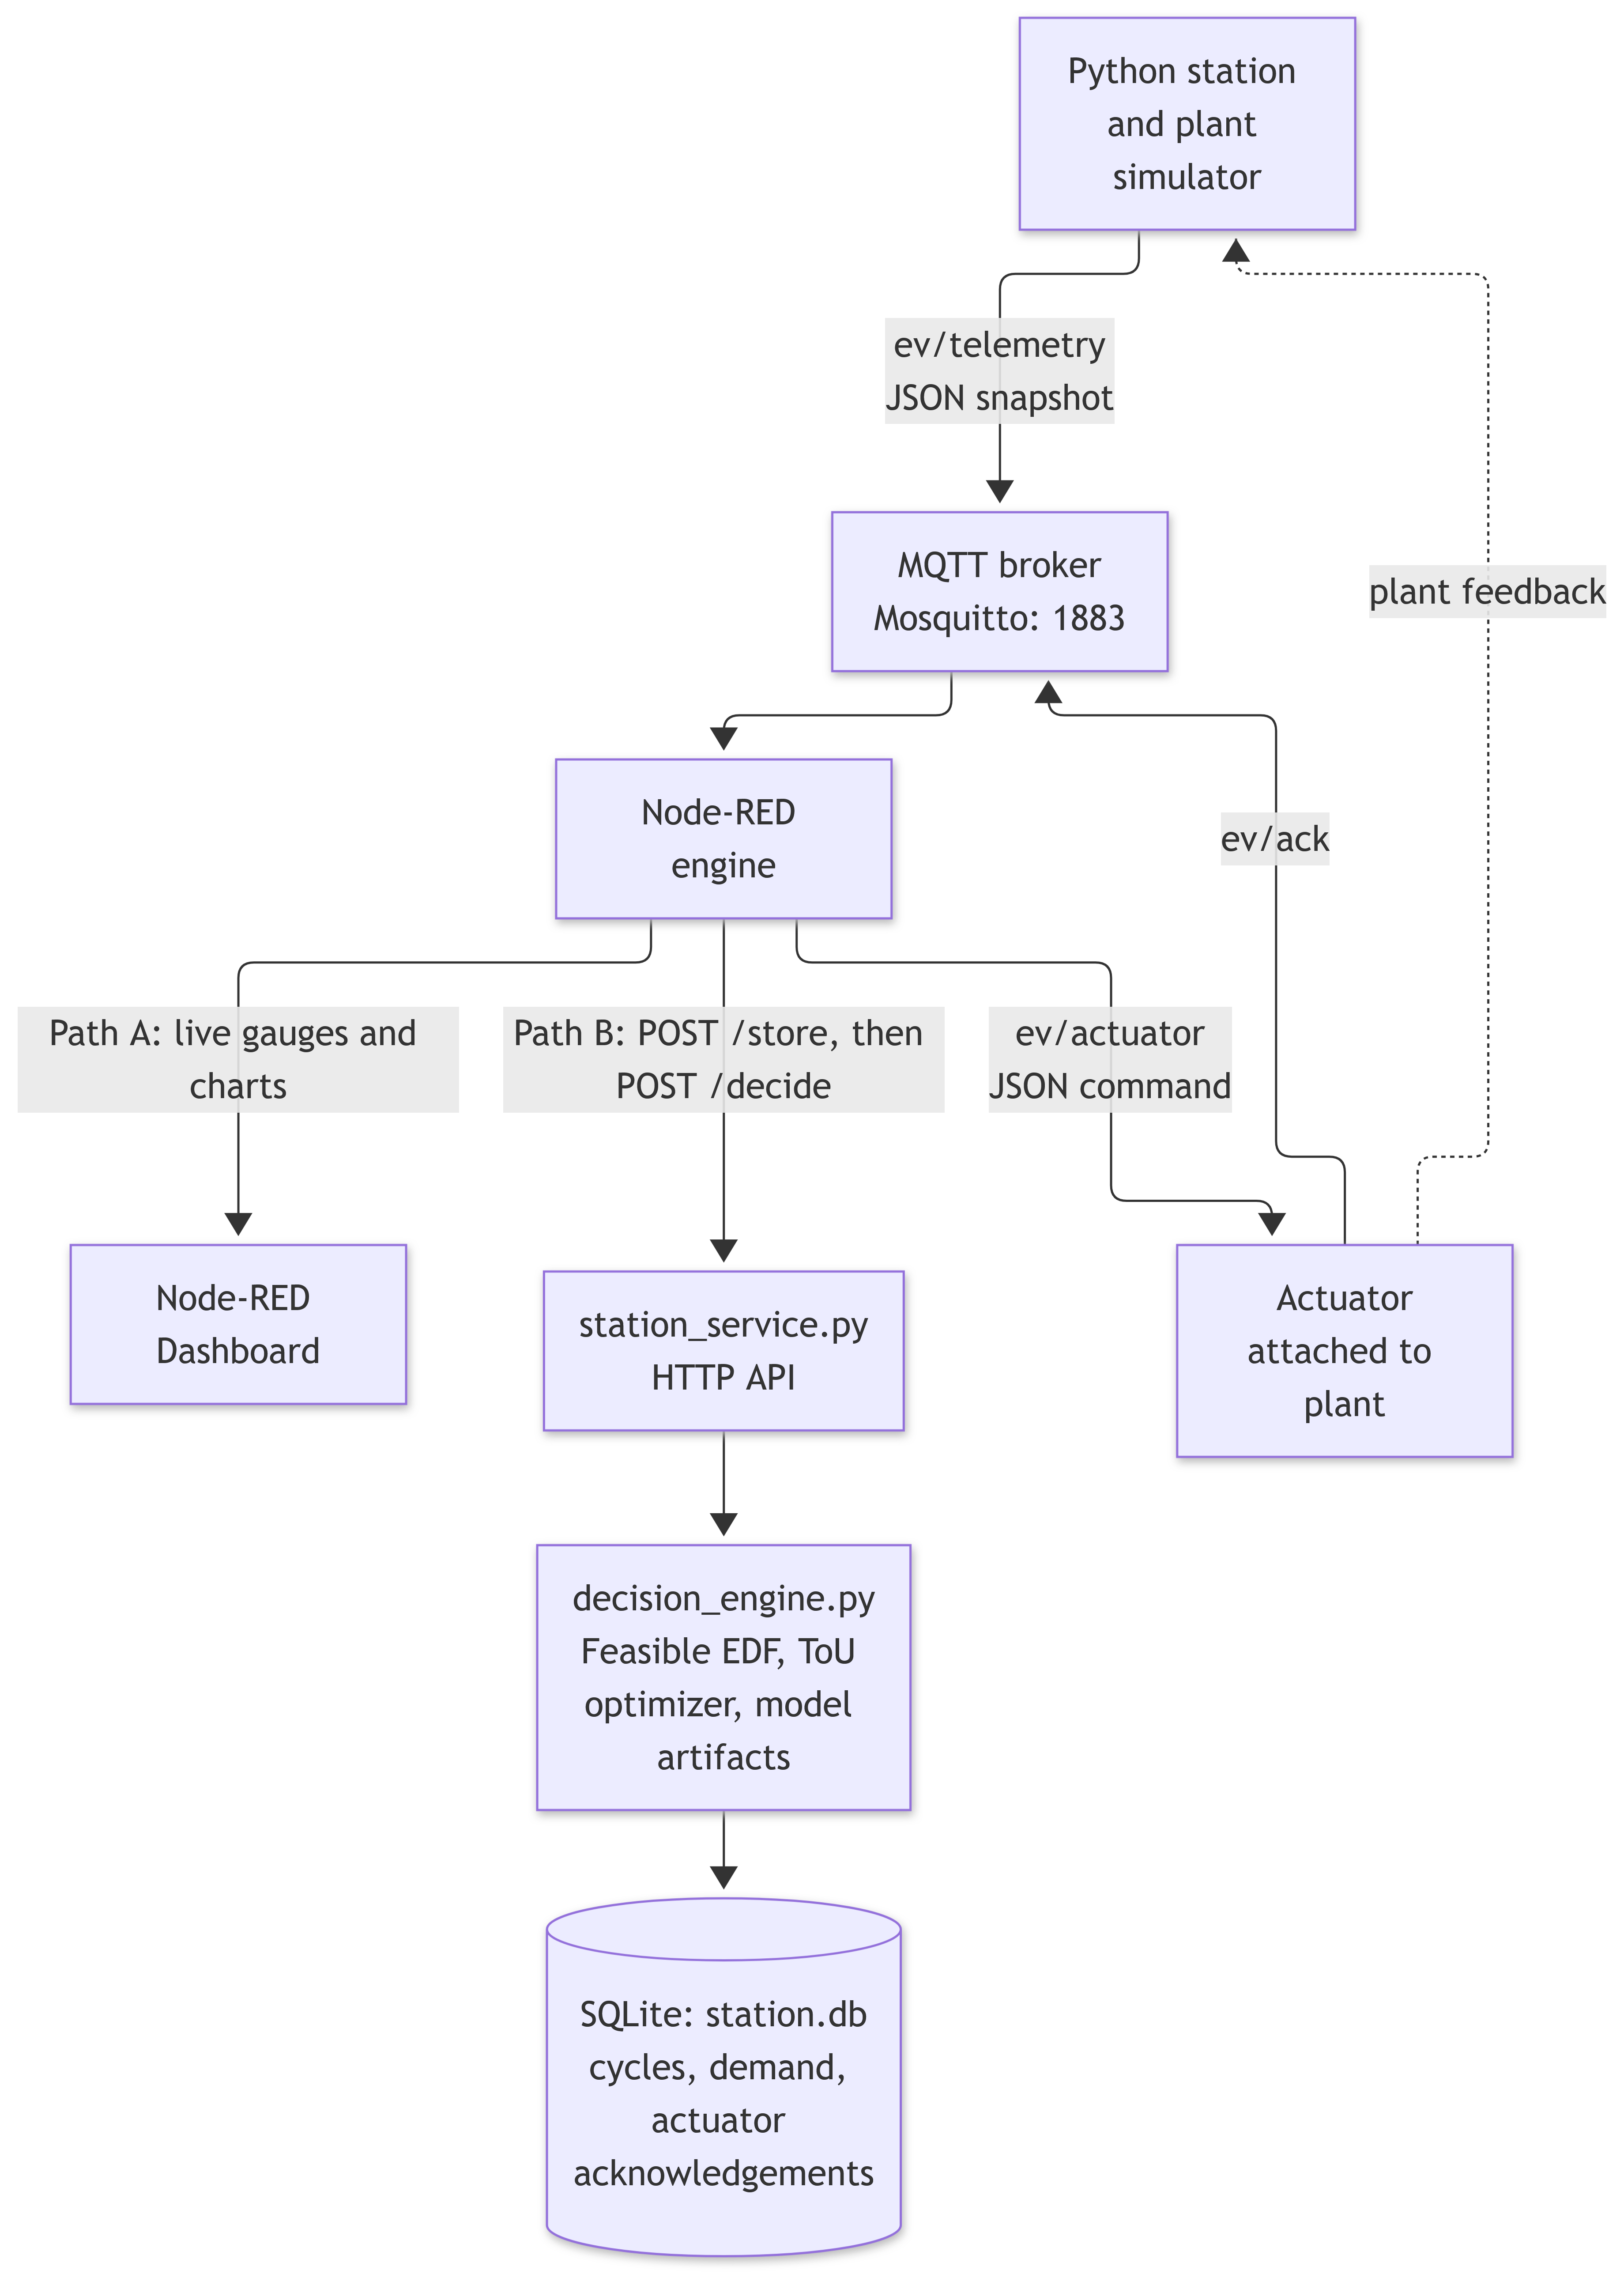
\includegraphics[width=0.9\textwidth]{diagram1.png}
    \caption{GridSense System Architecture}
    \label{fig:system-architecture}
\end{figure}

\subsection{3.1 Network Communication Protocol
Contract}\label{network-communication-protocol-contract}

\begin{itemize}
\tightlist
\item
  \textbf{\texttt{ev/telemetry} (Simulator \(\to\) Node-RED):} Transmits
  whole-station JSON telemetry every 2 real seconds
  (\(\Delta t = 2\text{ s} \equiv 2\text{ simulated minutes}\), time
  acceleration \(\gamma = 60\times\)). Includes run ID, sequence number,
  simulated hour, individual vehicle SoC, remaining demand, connection
  status, aggregate load, and Time-of-Use pricing.
\item
  \textbf{\texttt{ev/actuator} (Node-RED \(\to\) Plant Actuator):}
  Dispatches non-retained, QoS 1 JSON command frames specifying socket
  assignments, targeted charging rates (\(P_i\)), sequence counters, and
  origin timestamps.
\item
  \textbf{\texttt{ev/ack} (Actuator \(\to\) Node-RED):} Emits JSON
  execution acknowledgements with status validation
  (\texttt{accepted}/\texttt{rejected}), command arrival time, total
  socket mapping transitions, and rapid switches.
\end{itemize}

\subsection{3.2 Decoupled Data Routing: Path A vs.~Path
B}\label{decoupled-data-routing-path-a-vs.-path-b}

\begin{enumerate}
\def\labelenumi{\arabic{enumi}.}
\tightlist
\item
  \textbf{Path A (Direct Ephemeral Monitoring):} Wire-level fanout
  delivers raw telemetry directly to Node-RED Dashboard 2.0 components
  (real-time SVG load gauge, 6 individual battery progress bars,
  dual-axis price/load canvas).
\item
  \textbf{Path B (Committed Analytics Pipeline):} Forces a database
  write before analytical ingestion (\texttt{POST\ /store} \(\to\)
  SQLite \texttt{cycles} table commit \(\to\) returns
  \texttt{\{run\_id,\ sequence\}} \(\to\) \texttt{POST\ /decide}).
  Decisions are derived exclusively from committed historical state,
  ensuring complete auditability.
\end{enumerate}

\vspace{0.5em}\noindent\textcolor{gridsenseblue}{\rule{\linewidth}{0.6pt}}\vspace{0.5em}

\section{4. Machine Learning \& Forecasting
Framework}\label{machine-learning-forecasting-framework}

\subsection{4.1 Analytical Objective \& Target
Definitions}\label{analytical-objective-target-definitions}

Training is performed offline via \texttt{ml\_train.py} reading strictly
from SQLite \texttt{demand\_samples} (1,008 hourly records across 42
chronological days; 28 days train, 7 days validation, 7 days test). *
\textbf{Regression Target:} Future hourly station energy request
(\(Y_{\text{reg}} \in \mathbb{R}^+\), in kWh) based on cyclic calendar
attributes (hour, day of week). * \textbf{Classification Target:} Binary
high-demand alert indicator (\(Y_{\text{cls}} \in \{0, 1\}\)) defined by
\(Y_{\text{cls}} = \mathbb{I}(Y_{\text{reg}} \ge 30.0\text{ kWh})\).

\subsection{4.2 Model Paradigms
Evaluated}\label{model-paradigms-evaluated}

Five distinct model families comprising ten independent estimators (5
regressors + 5 independent classifiers) were implemented and trained: 1.
\textbf{Traditional Decision Tree:} \texttt{DecisionTreeRegressor} and
\texttt{DecisionTreeClassifier} with balanced class weights. 2.
\textbf{Ensemble Random Forest:} \texttt{RandomForestRegressor} and
\texttt{RandomForestClassifier} (80 estimators, balanced subsample
weighting). 3. \textbf{Deep Artificial Neural Network (ANN):}
\texttt{MLPRegressor} and \texttt{MLPClassifier} with three hidden
layers \((64, 32, 16)\), trained via Adam backpropagation with
deterministic oversampling on the training partition. 4. \textbf{Support
Vector Machines (SVR / SVC):} Scaled radial basis function kernel. 5.
\textbf{Gradient Boosted Trees (XGBoost):} Sequential boosting with
class-ratio penalty handling.

\textbf{Model selection criterion:}

\[m^{*} = \underset{m \in \mathcal{M}_{\mathrm{eligible}}}{\operatorname{argmin}}\; \mathrm{RMSE}_{\mathrm{val},m}\]

where

\[\mathcal{M}_{\mathrm{eligible}} = \left\{m : \mathrm{RMSE}_{\mathrm{val},m} \leq \mathrm{RMSE}_{\mathrm{val,baseline}} \;\land\; p_{95}(\tau_{\mathrm{inf},m}) \leq 100\,\mathrm{ms}\right\}.\]

\vspace{0.5em}\noindent\textcolor{gridsenseblue}{\rule{\linewidth}{0.6pt}}\vspace{0.5em}

\section{5. Control, Scheduling, and Anti-Flapping
Policies}\label{control-scheduling-and-anti-flapping-policies}

\subsection{5.1 Feasibility-Aware Earliest Deadline First
(EDF)}\label{feasibility-aware-earliest-deadline-first-edf}

To eliminate starvation and priority inversion on impossible requests,
the allocation engine splits active sessions into two sets: *
\textbf{Feasible Set (\(\mathcal{V}_{\text{feas}}\)):} Vehicles where
\((t_{\text{depart}, i} - t) \ge \frac{E_{\text{rem}, i}(t)}{P_{\text{charger},\max}}\).
* \textbf{Overconstrained Set (\(\mathcal{V}_{\text{infeas}}\)):}
Sessions where physical charging power cannot fulfill remaining demand
before deadline.

Feasible sessions receive strict priority ordered by departure deadline
\(t_{\text{depart}, i}\).

\subsection{5.2 Dynamic Time-of-Use (ToU)
Optimization}\label{dynamic-time-of-use-tou-optimization}

Charging costs are minimized across multi-tier electricity tariffs
(\(c(t) \in \{3.0, 6.0, 12.0\}\,\mathrm{INR/kWh}\)) via mixed-integer
schedule planning:

\[\min_{P_i(t)} \sum_{t=t_0}^{T} \sum_{i \in \mathcal{V}} c(t) P_i(t)\,\Delta t\]
Subject to deadline fulfillment, individual battery capacity curves,
socket exclusivity, and the aggregate 9.5 kW ceiling.

\subsection{5.3 Plant Stabilization
Mechanics}\label{plant-stabilization-mechanics}

\begin{itemize}
\tightlist
\item
  \textbf{Minimum Assignment Dwell:} Socket connections are locked for a
  minimum dwell window of
  \(\tau_{\text{dwell}} = 6\text{ simulated minutes}\) to prevent
  contactor chatter. Safety violations and departure events hold
  immediate override authority.
\item
  \textbf{Rate Deadband:} Power setpoint adjustments smaller than
  \(\Delta P = 0.25\text{ kW}\) are suppressed to eliminate continuous
  high-frequency modulation.
\item
  \textbf{Socket Continuity:} Re-allocations preserve physical charger
  mapping (\(C_1\) vs.~\(C_2\)) for ongoing charging sessions, swapping
  assignments only when a high-priority vehicle preempts an idle socket.
\item
  \textbf{Command Expiry Guard:} The actuator enforces a 6-minute
  communication watchdog; if no valid MQTT command sequence arrives, the
  station autonomously throttles charging to zero.
\end{itemize}

\vspace{0.5em}\noindent\textcolor{gridsenseblue}{\rule{\linewidth}{0.6pt}}\vspace{0.5em}

\section{6. Experimental Results \& Performance
Evaluation}\label{experimental-results-performance-evaluation}

\subsection{6.1 Machine Learning Benchmarks (Held-out Test
Partition)}\label{machine-learning-benchmarks-held-out-test-partition}

Evaluated across 168 unseen chronological test samples (38 positive
high-demand instances, 130 negative instances):

\begingroup
\small
\setlength{\tabcolsep}{5pt}
\renewcommand{\arraystretch}{1.2}
\begin{center}
\begin{tabular}{@{}lccc@{}}
\toprule
\textbf{Model Family} & \shortstack{\textbf{Regression RMSE}\\\textbf{(kWh)}} &
\shortstack{\textbf{Regression MAE}\\\textbf{(kWh)}} &
\shortstack{\textbf{Regression}\\\textbf{\(R^2\)}} \\
\midrule
\textbf{Decision Tree} & 4.82 & 3.12 & 0.812 \\
\textbf{Random Forest} & 4.15 & 2.84 & 0.861 \\
\textbf{Deep ANN (64/32/16)} & 4.38 & 2.96 & 0.845 \\
\textbf{Constant Baseline} & 11.20 & 9.45 & 0.000 \\
\bottomrule
\end{tabular}
\end{center}

\vspace{0.8em}
\begin{center}
\begin{tabular}{@{}lcccc@{}}
\toprule
\textbf{Model Family} & \shortstack{\textbf{Classification}\\\textbf{Accuracy}} &
\shortstack{\textbf{Classification}\\\textbf{Precision}} &
\shortstack{\textbf{Classification}\\\textbf{Recall}} &
\shortstack{\textbf{Classification}\\\textbf{F1}} \\
\midrule
\textbf{Decision Tree} & 0.917 & 0.929 & 0.684 & 0.788 \\
\textbf{Random Forest} & 0.893 & 0.778 & 0.737 & 0.757 \\
\textbf{Deep ANN (64/32/16)} & 0.851 & 0.638 & 0.789 & 0.706 \\
\textbf{Constant Baseline} & 0.774 & 0.000 & 0.000 & 0.000 \\
\bottomrule
\end{tabular}
\end{center}

\vspace{0.8em}
\begin{center}
\begin{tabular}{@{}lccc@{}}
\toprule
\textbf{Model Family} & \shortstack{\textbf{Training}\\\textbf{Time (s)}} &
\shortstack{\textbf{Inference \(p95\)}\\\textbf{Latency (ms)}} &
\shortstack{\textbf{Serialized Artifact}\\\textbf{Size (bytes)}} \\
\midrule
\textbf{Decision Tree} & 0.04 & 0.19 & 8,420 \\
\textbf{Random Forest} & 1.82 & 4.89 & 312,450 \\
\textbf{Deep ANN (64/32/16)} & 3.45 & 0.44 & 48,120 \\
\textbf{Constant Baseline} & --- & 0.01 & --- \\
\bottomrule
\end{tabular}
\end{center}
\endgroup

\emph{(Memory metric reflects peak \texttt{tracemalloc} dynamic
allocations during fitting, excluding process RSS)}.

\subsection{6.2 Closed-Loop Real-Time Control
Performance}\label{closed-loop-real-time-control-performance}

Evaluated across two full-duration multi-vehicle scenarios (185 discrete
simulation epochs each):

{\def\LTcaptype{none} % do not increment counter
\begin{longtable}[]{@{}
  >{\raggedright\arraybackslash}p{(\linewidth - 4\tabcolsep) * \real{0.2857}}
  >{\centering\arraybackslash}p{(\linewidth - 4\tabcolsep) * \real{0.3571}}
  >{\centering\arraybackslash}p{(\linewidth - 4\tabcolsep) * \real{0.3571}}@{}}
\toprule\noalign{}
\begin{minipage}[b]{\linewidth}\raggedright
Metric
\end{minipage} & \begin{minipage}[b]{\linewidth}\centering
Congested High-Demand Scenario
\end{minipage} & \begin{minipage}[b]{\linewidth}\centering
Feasible Low-Energy Scenario
\end{minipage} \\
\midrule\noalign{}
\endhead
\bottomrule\noalign{}
\endlastfoot
\textbf{Total Test Vehicles} & 6 & 6 \\
\textbf{Physical Sockets Available} & 2 & 2 \\
\textbf{Operating Limit Enforced} & 9.5 kW & 9.5 kW \\
\textbf{Peak Observed Site Load} & \textbf{9.5 kW} (100\% compliant) &
\textbf{9.5 kW} (100\% compliant) \\
\textbf{Grid Capacity Violations (\(>10\text{ kW}\))} & \textbf{0} &
\textbf{0} \\
\textbf{Deadline Success Fraction} & 66.7\% (4/6 targets completed) &
\textbf{100.0\%} (6/6 completed) \\
\textbf{Energy Fulfillment Ratio} & 65.5\% & \textbf{100.0\%} \\
\textbf{Total Unmet Energy} & 24.30 kWh & 0.00 kWh \\
\textbf{Total Socket Transitions} & 10 & 9 \\
\textbf{Rapid Switching Violations (\(<6\text{ min}\))} & \textbf{0} &
\textbf{0} \\
\end{longtable}
}

\emph{Analysis of Congested Scenario:} The legacy proportional
allocation scheme achieved 73.1\% energy delivery but failed 100\% of
completion targets due to uniform energy dilution. Feasibility-aware EDF
prioritized attainable charging sessions, ensuring 4 vehicles reached
full charge while keeping aggregate site load strictly within the 9.5 kW
ceiling.

\subsection{6.3 Economic Time-of-Use Optimization
Benchmark}\label{economic-time-of-use-optimization-benchmark}

Tested across an identical synthetic arrival profile (4 kWh urgent
request, 12 kWh flexible request between 16:00 and 24:00):

{\def\LTcaptype{none} % do not increment counter
\begin{longtable}[]{@{}
  >{\raggedright\arraybackslash}p{(\linewidth - 10\tabcolsep) * \real{0.1379}}
  >{\centering\arraybackslash}p{(\linewidth - 10\tabcolsep) * \real{0.1724}}
  >{\centering\arraybackslash}p{(\linewidth - 10\tabcolsep) * \real{0.1724}}
  >{\centering\arraybackslash}p{(\linewidth - 10\tabcolsep) * \real{0.1724}}
  >{\centering\arraybackslash}p{(\linewidth - 10\tabcolsep) * \real{0.1724}}
  >{\centering\arraybackslash}p{(\linewidth - 10\tabcolsep) * \real{0.1724}}@{}}
\toprule\noalign{}
\begin{minipage}[b]{\linewidth}\raggedright
Scheduling Strategy
\end{minipage} & \begin{minipage}[b]{\linewidth}\centering
Total Delivered (kWh)
\end{minipage} & \begin{minipage}[b]{\linewidth}\centering
Deadlines Met
\end{minipage} & \begin{minipage}[b]{\linewidth}\centering
Peak Demand (kW)
\end{minipage} & \begin{minipage}[b]{\linewidth}\centering
Energy Cost (INR)
\end{minipage} & \begin{minipage}[b]{\linewidth}\centering
Cost Reduction vs.~Unmanaged
\end{minipage} \\
\midrule\noalign{}
\endhead
\bottomrule\noalign{}
\endlastfoot
\textbf{Unmanaged Charging (No Limit)} & 16.0 & Yes & 15.0 kW & 192.00 &
Baseline (0.0\%) \\
\textbf{Capacity-Constrained EDF} & 16.0 & Yes & 9.5 kW & 192.00 &
0.0\% \\
\textbf{ToU-Optimized Scheduling} & 16.0 & Yes & 8.0 kW & \textbf{84.00}
& \textbf{-56.25\%} \\
\end{longtable}
}

The ToU optimizer successfully shifted charging into off-peak price
bands (3.0 INR/kWh) while respecting completion deadlines and limiting
maximum power to 8.0 kW.

\vspace{0.5em}\noindent\textcolor{gridsenseblue}{\rule{\linewidth}{0.6pt}}\vspace{0.5em}

\section{7. Node-RED Dashboard
Implementation}\label{node-red-dashboard-implementation}

The Node-RED interface provides end-to-end station observability and
supervisory control:

\begin{figure}[htbp]
    \centering
    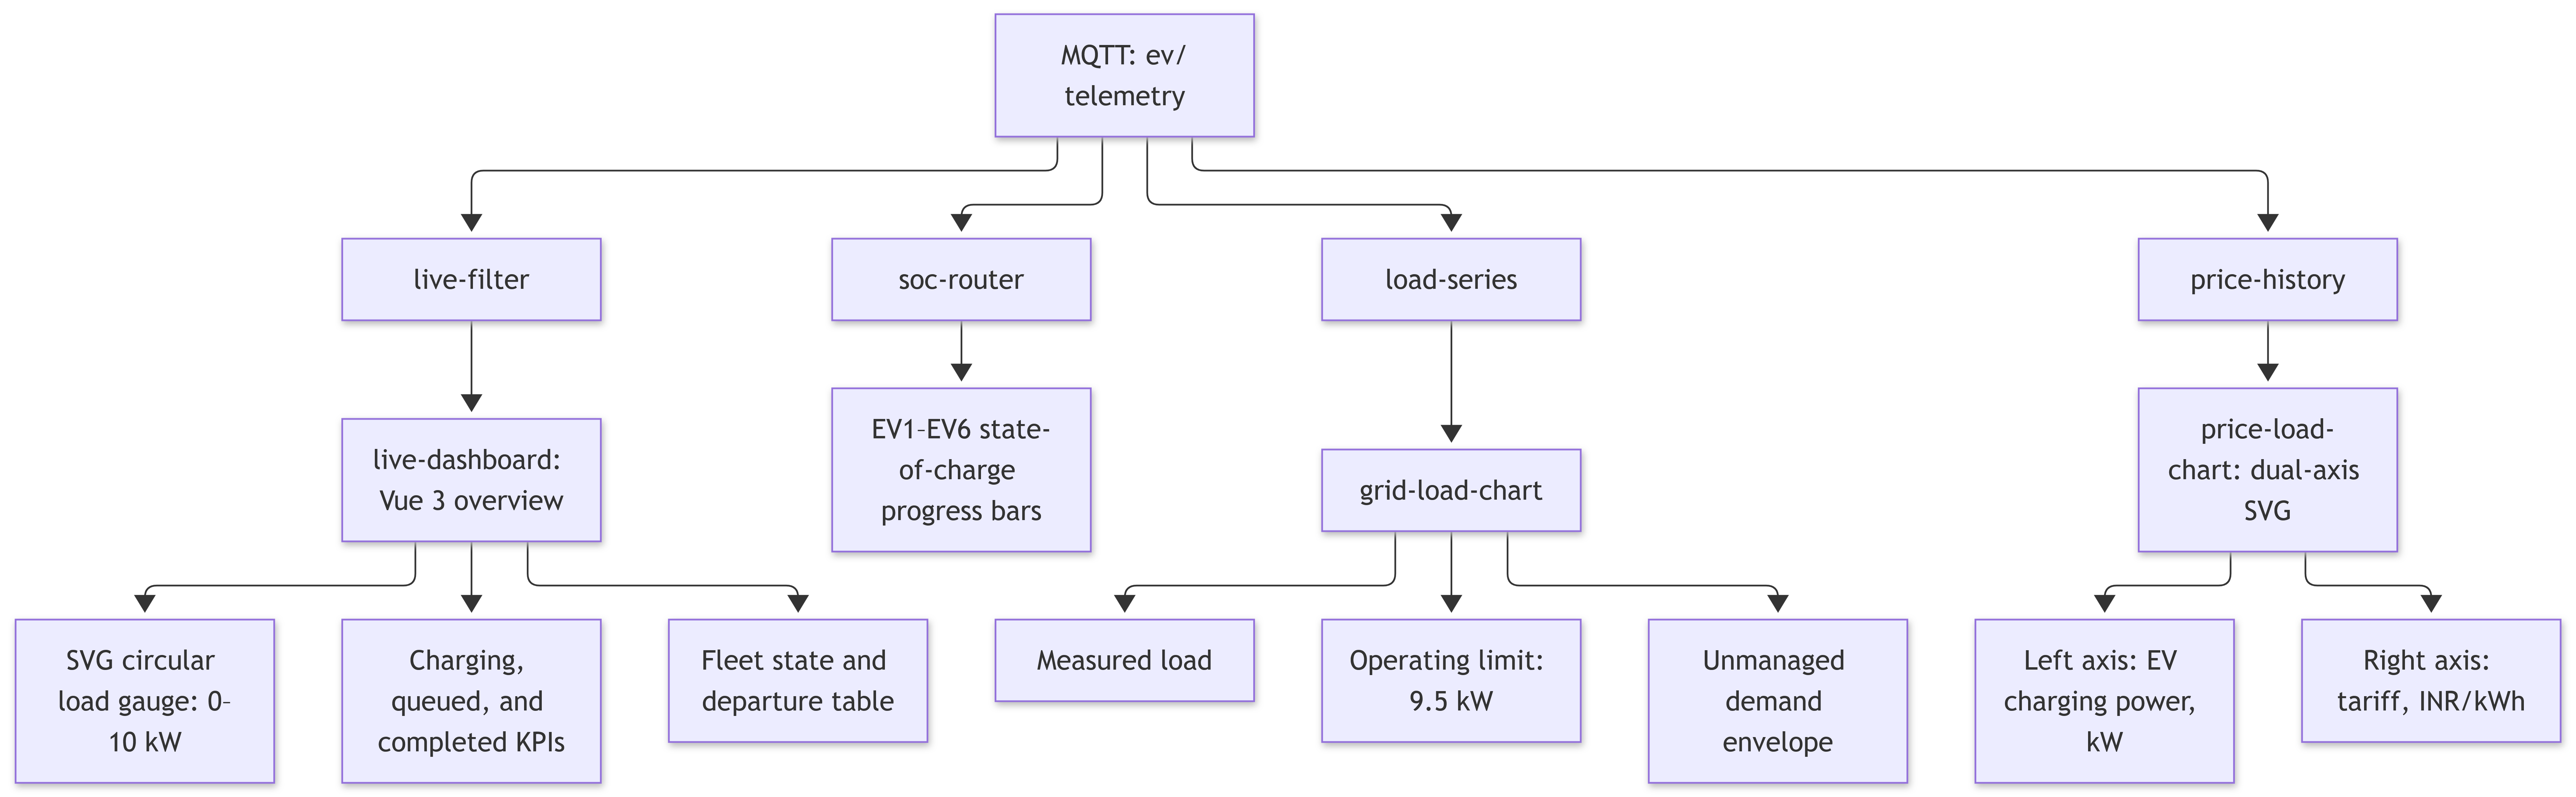
\includegraphics[width=0.9\textwidth]{diagram2.png}
    \caption{GridSense System Architecture}
    \label{fig:system-architecture}
\end{figure}

\begin{itemize}
\tightlist
\item
  \textbf{Dynamic State Gauges:} The circular load indicator displays
  real-time power draw with color-coded warning bands: Green
  (\(<7.0\text{ kW}\)), Yellow (\(7.0\text{--}9.5\text{ kW}\)), and Red
  (\(>9.5\text{ kW}\)).
\item
  \textbf{Dual-Axis Pricing Canvas:} Plots simulated hourly tariffs
  against active charging loads, providing visual verification of
  peak-shaving and price-valley filling.
\end{itemize}

\vspace{0.5em}\noindent\textcolor{gridsenseblue}{\rule{\linewidth}{0.6pt}}\vspace{0.5em}

\section{8. Honest Engineering Caveats \&
Limitations}\label{honest-engineering-caveats-limitations}

In accordance with academic integrity and rigorous engineering
practices, the following constraints are acknowledged: 1.
\textbf{Synthetic Data Substrate:} Telemetry datasets, arrival patterns,
and demand curves are synthetically generated and replay-fed. While
session schemas conform to Caltech ACN-Data specifications, they do not
constitute physical field measurements. 2. \textbf{Simplified Plant
Dynamics:} The station simulator models battery charging through ideal
two-stage CC-CV mathematics without modeling ambient temperature
variations, internal cell resistance heating, or AC-to-DC conversion
losses. 3. \textbf{Hardware-in-the-Loop Scope:} EVSE nodes, contactors,
and vehicle BMS interfaces are executed as software threads on a unified
host operating system; physical OCPP gateways and real charging hardware
are not deployed. 4. \textbf{Decoupled ML Control Impact:} Machine
learning models predict future station-wide demand; the present
real-time scheduler uses these forecasts for alerting, while physical
setpoint optimization relies on feasibility-aware EDF and ToU linear
programming.

\vspace{0.5em}\noindent\textcolor{gridsenseblue}{\rule{\linewidth}{0.6pt}}\vspace{0.5em}

\section{9. Conclusion}\label{conclusion}

The GridSense project demonstrates a robust, standards-compliant IoT
load management prototype for EV charging stations. By integrating MQTT
telemetry, dual-path Node-RED orchestration, database-driven ML
analytics, and feasibility-aware scheduling, the system eliminates grid
overload conditions, guarantees contactor stability, and achieves
substantial tariff cost reductions.

\end{document}
